% Generated by `uv run analyze`; needs \usepackage{pgfplots}
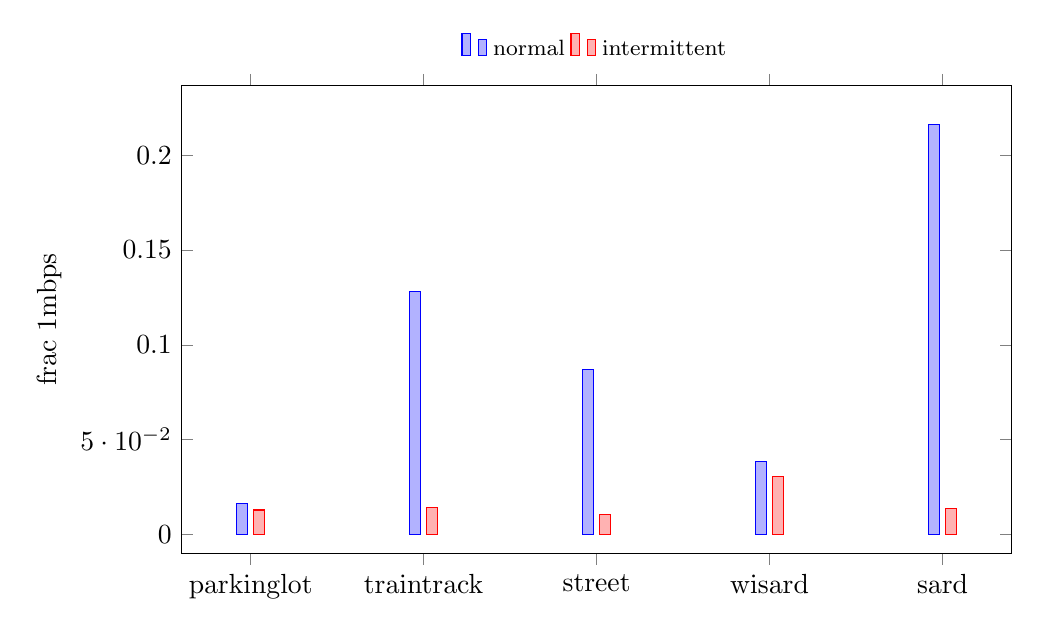
\begin{tikzpicture}
\begin{axis}[ybar, width=\columnwidth, height=0.62\columnwidth, bar width=4pt,
  symbolic x coords={parkinglot,traintrack,street,wisard,sard}, xtick=data, ylabel={frac 1mbps},
  legend style={at={(0.5,1.03)}, anchor=south, legend columns=-1, draw=none, font=\footnotesize},
  error bars/y dir=both, error bars/y explicit]
\addplot coordinates {(parkinglot,0.01628) +- (0,0) (traintrack,0.1279) +- (0,0) (street,0.08692) +- (0,0) (wisard,0.03841) +- (0,0) (sard,0.2161) +- (0,0)};
\addlegendentry{normal}
\addplot coordinates {(parkinglot,0.01284) +- (0,0) (traintrack,0.0141) +- (0,0) (street,0.01061) +- (0,0) (wisard,0.03064) +- (0,0) (sard,0.01365) +- (0,0)};
\addlegendentry{intermittent}
\end{axis}
\end{tikzpicture}
